\chapter{线性化、共振面与外区驱动力}\label{tm:linear}
\section{什么是线性模，为什么用复指数}
设平衡量只依赖$x$，扰动沿$y$周期变化。用一个小参数$\epsilon_p$记录振幅阶数：
\begin{align}
 \psi(x,y,t)&=\psi_0(x)+\epsilon_p\operatorname{Re}\{\Psi(x)e^{iky+\gamma t}\},\\
 \phi(x,y,t)&=\epsilon_p\operatorname{Re}\{\Phi_c(x)e^{iky+\gamma t}\}.
 \label{tm:ansatz}
\end{align}
$\epsilon_p$与内层尺度$\delta/a$不是同一小参数。线性化只保留$O(\epsilon_p)$，删去两个扰动相乘的$O(\epsilon_p^2)$项。复数只是方便的记号，因为对一个模而言$\partial_y\to ik$、$\partial_t\to\gamma$；真实场总取实部。一般$\gamma$可为复数，实部代表增长，虚部代表相位传播。先研究静态对称平衡中的纯增长支$\gamma>0$，并不否认实验模会旋转。

定义
\begin{equation}
 F(x)\equiv\psi_0'(x)=B_{0y}(x),\qquad
 \mathcal L_k\equiv\frac{\dd^2}{\dd x^2}-k^2.
\end{equation}
本章撇号始终表示对有量纲$x$求导，故$F'$单位$\mathrm{T/m}$，$\Psi'$单位T。下一章若改用$X=x/a$会重新标明。

\section{磁通方程的线性化：把四项展开}
泊松括号展开为
\begin{equation}
 [\phi,\psi]=[0,\psi_0]+[\phi_1,\psi_0]+[0,\psi_1]+[\phi_1,\psi_1].
\end{equation}
第一、三项为零，最后一项为二阶小量。由于$\partial_y\psi_0=0$，中间保留项为
\begin{equation}
 [\phi_1,\psi_0]=(\partial_x\phi_1)\underbrace{\partial_y\psi_0}_{0}
 -(\partial_y\phi_1)\partial_x\psi_0=-ikF\Phi_c e^{iky+\gamma t}.
\end{equation}
背景扩散属于零阶平衡方程，扣除背景后得到
\begin{equation}
 \boxed{\gamma\Psi=ikF\Phi_c+D_\eta\mathcal L_k\Psi.}
 \label{tm:linind}
\end{equation}
这里保留了$k^2\Psi$。在薄内层中稍后可以通过$k\delta\ll1$删除它；\textbf{在外区不能提前删掉}，否则会丢失远处衰减与波长稳定阈值。

\section{涡量方程的线性化：电流梯度从哪里来}
因为平衡流为零，左侧非线性平流$[\phi,\nabla^2\phi]$完全是二阶。右侧有两项一阶贡献：
\begin{align}
 [\psi,\nabla^2\psi]_1
 &=[\psi_0,\nabla^2\psi_1]+[\psi_1,\nabla^2\psi_0],\\
 [\psi_0,\nabla^2\psi_1]&=F\,ik\mathcal L_k\Psi\,e^{iky+\gamma t},\\
 [\psi_1,\nabla^2\psi_0]&=-ik\Psi\,\frac{\dd}{\dd x}(\psi_0'')e^{iky+\gamma t}
 =-ikF''\Psi e^{iky+\gamma t}.
\end{align}
于是
\begin{equation}
 \boxed{\gamma\mathcal L_k\Phi_c
 =\frac{ik}{\mu_0\rho}\left(F\mathcal L_k\Psi-F''\Psi\right).}
 \label{tm:linvort}
\end{equation}
$F''=\mu_0J_{0z}'$正是平衡电流梯度信息。若只保留$F\Psi''$而把$F''\Psi$到处删除，就不能正确计算外区驱动力。近片中心的内层可因局部线性磁剪切忽略$F''$；这个局部事实不能推广到整个电流片。

对于纯增长的对称撕裂支，可令$\Psi$为实函数并写$\Phi_c=-i\Phi$，其中$\Phi$也为实函数。这对应磁通扰动为$\Psi\cos ky$，流函数为$\Phi\sin ky$。代入后得到实方程
\begin{align}
 \gamma\Psi&=kF\Phi+D_\eta\mathcal L_k\Psi,\label{tm:realind}\\
 \gamma\mathcal L_k\Phi&=-\frac{k}{\mu_0\rho}
 \left(F\mathcal L_k\Psi-F''\Psi\right).
 \label{tm:realvort}
\end{align}
第二式的负号来自将两边共同的$i$约去，而不是任意选择。对于奇函数$F$，撕裂支的$\Psi(x)$为偶函数、$\Phi(x)$为奇函数；两侧流动围绕磁岛有相应奇偶性。

\section{共振面为什么是内外区分界}
沿平衡磁场对一个扰动求导：
\begin{equation}
 \B_0\cdot\nabla(\widetilde f e^{iky+ik_zz})
 =i(kF+k_zB_g)\widetilde f e^{iky+ik_zz}.
\end{equation}
磁张力沿场传递，因而$kF+k_zB_g=0$处的沿场恢复作用有特殊性；此处称共振面。在本讲义的二维$k_z=0$问题中，共振面就是$F=0$，对Harris片为$x=0$。有导场并不使这一二维共振面消失；若允许斜模$k_z\ne0$，共振面位置就会改变。

设外区电阻很小，先从式\eqref{tm:realind}得到
\begin{equation}
 \Phi\simeq\frac{\gamma\Psi}{kF}.
 \label{tm:idealflow}
\end{equation}
如果$\Psi(0)\ne0$且$F\simeq B'_0x$，这个理想解在$x\to0$时像$1/x$发散。这并不是实际流速无限大，而是告诉我们：\textbf{删掉电阻的近似在这里失效}。小电阻乘上很大的磁通二阶导数，仍可以与时间项同阶。薄层内还必须保留惯性，否则无法决定增长时标。这就是奇异摄动，而不是在全域给理想解简单加一个很小修正。

\paragraph{类比，但只作理解。}
在一根几乎没有电阻的导线上，绝大部分电压降可以集中在一个很短的电阻段；“段很短”不等于“段不重要”。撕裂内层同样可以很薄，却决定拓扑改变与增长率。外区仍不可省略，因为它决定有多少自由能和何种边界响应能供给内层。

\section{外区近似的时间排序}
令$\tau_A=a/V_A$、$\tau_R=a^2/D_\eta$，假设
\begin{equation}
 \tau_A\ll\gamma^{-1}\ll\tau_R,
 \qquad\text{即}\qquad S_a^{-1}\ll\hat\gamma\ll1,
 \quad \hat\gamma\equiv\gamma\tau_A.
 \label{tm:outerordering}
\end{equation}
右边不等式使外区在模明显增长之前已能近似完成Alfv\'en力平衡；左边不等式使背景尚未显著电阻扩散。若沿片波数很小，还须检查模相对于沿片Alfv\'en时间的慢排序$\gamma\ll kV_A$，不能只检查$\hat\gamma\ll1$。

在$|x|\sim a$，$\mathcal L_k\sim a^{-2}$（$ka=O(1)$）且由式\eqref{tm:idealflow}，$\Phi\sim\gamma\Psi/(kB_0)$。惯性与磁力之比估计为
\begin{equation}
 \frac{\gamma\Phi/a^2}{kB_0\Psi/(\mu_0\rho a^2)}
 \sim\frac{\gamma^2\mu_0\rho}{k^2B_0^2}
 =\left(\frac{\gamma}{kV_A}\right)^2\ll1.
\end{equation}
因此外区涡量式右端应近似为零：
\begin{equation}
 F(\Psi''-k^2\Psi)-F''\Psi=0.
\end{equation}
在$F\ne0$处除以$F$，得到\emph{外区撕裂方程}
\begin{equation}
 \boxed{\Psi''-\left(k^2+\frac{F''}{F}\right)\Psi=0.}
 \label{tm:outerode}
\end{equation}
它是二阶常微分方程，不含$\gamma$，所以\textbf{外区本身决定不了增长率}。它计算的是近似静态磁力平衡对薄层磁通扰动的响应。\citep{TMFitzMatching}

\section{\texorpdfstring{$\Delta'$}{Delta prime}的定义：比较的是两侧斜率}
分别在$x>0$与$x<0$解式\eqref{tm:outerode}，要求远离电流片时扰动衰减（或满足实际壁面条件）。由于线性问题的总振幅任意，可以把两侧解都归一成$\Psi(0)=\Psi_s$。两侧函数值相同，但外区延拓到零点后的导数一般不同。定义
\begin{equation}
 \boxed{\Delta'\equiv
 \frac{\Psi'(0^+)-\Psi'(0^-)}{\Psi_s}.}
 \label{tm:deltaprime}
\end{equation}
这里$0^\pm$是\emph{外区解向薄层中心的渐近延拓}，并不说真实磁场在中心有物理无限薄的不连续面。真实内区将这处斜率差平滑连接。$\Delta'$单位为$\mathrm{m^{-1}}$，$\Delta'a$才无量纲。

在重叠区$\delta\ll|x|\ll a$，偶对称解具有
\begin{equation}
 \Psi_{\rm out}(x)=\Psi_s\left(1+\frac{\Delta'}{2}|x|+\cdots\right).
 \label{tm:outermatch}
\end{equation}
内区解的远场也必须给出相同常数项与线性斜率。这一“相同区域中表示同一个函数”的要求叫渐近匹配。不能把两条图线在任选一点简单接起来当成匹配。

还可用积分读出$\Delta'$：跨过内层，
\begin{equation}
 \int_{-\ell}^{\ell}\Psi''\,\dd x
 =\Psi'(\ell)-\Psi'(-\ell)\longrightarrow\Delta'\Psi_s,
 \quad \delta\ll\ell\ll a.
 \label{tm:currentjump}
\end{equation}
由$\mu_0\widetilde J_z=\Psi''-k^2\Psi$，它约束薄层中扰动电流的积分。$k^2$项的积分相对薄层二阶导数项为小量，删除它须依赖薄层排序。

在这里研究的经典静态、无压强曲率驱动、无流剪切电阻问题中，$\Delta'>0$给出不稳定撕裂支；$\Delta'<0$没有该自发增长支。这个结论不能无条件推广到新经典撕裂模、受迫重联、漂移或流剪切驱动问题。负$\Delta'$的系统仍可被外部共振磁扰动强迫产生磁岛。

\begin{figure}[htbp]
\centering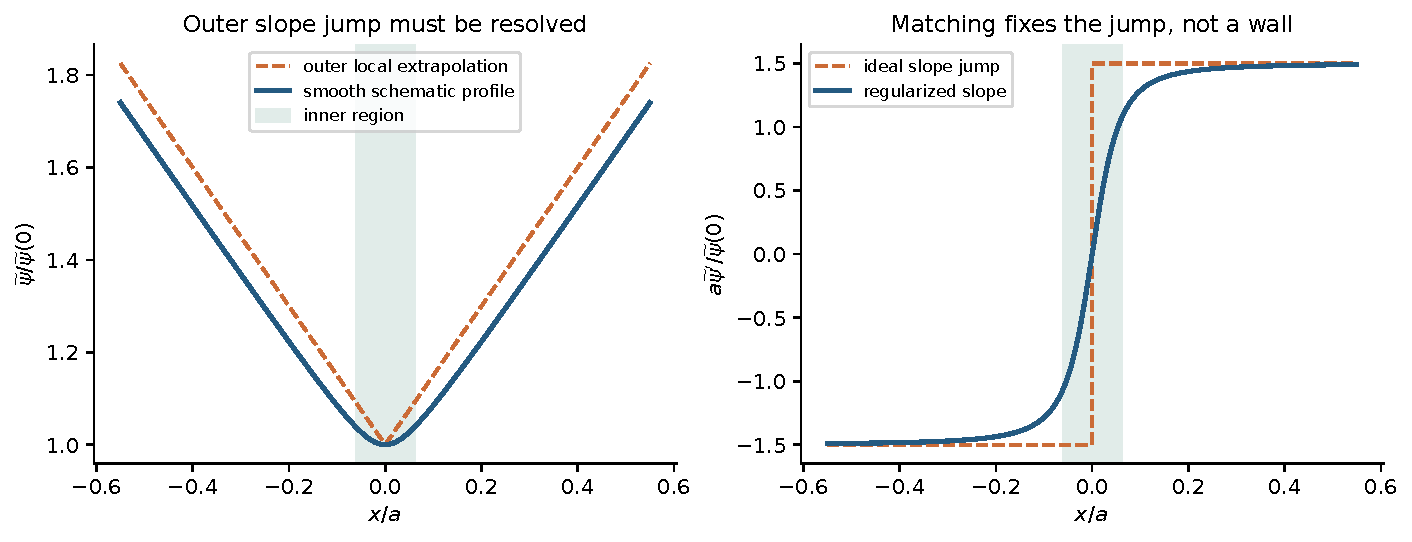
\includegraphics[width=\textwidth]{figures/tm_matching.pdf}
\caption{内外区匹配的几何示意，选取$\Delta'a=3$与$\delta/a=0.06$。红色曲线是为了展示“相同远场斜率、不同内层平滑”而构造的正则化函数，不是已求解的FKR内区本征函数，不能从图中读出精确层宽或增长率。}
\label{tm:fig:matching}
\end{figure}

\section{Harris片的外区解：从候选函数逐项验算}
对$F=B_0\tanh(x/a)$，令$X=x/a$、$K=ka$。因为
\begin{align}
 F'&=\frac{B_0}{a}\operatorname{sech}^2X,\\
 F''&=-\frac{2B_0}{a^2}\operatorname{sech}^2X\tanh X,
\end{align}
所以$F''/F=-2\operatorname{sech}^2X/a^2$。在$X=0$，分子与分母都趋零，但这个比值有有限极限；不要把形式上的$0/0$误认为外区系数必有无穷大。

式\eqref{tm:outerode}变为
\begin{equation}
 \frac{\dd^2\Psi}{\dd X^2}-\left(K^2-2\operatorname{sech}^2X\right)\Psi=0.
 \label{tm:harrisode}
\end{equation}
在$X>0$试取会在无穷远衰减的函数
\begin{equation}
 f_+(X)=e^{-KX}(K+\tanh X).
\end{equation}
为避免一行带过，令$T=\tanh X$、$Q=\operatorname{sech}^2X=1-T^2$，则$T'=Q$、$Q'=-2TQ$。两次求导：
\begin{align}
 f_+'&=e^{-KX}\{Q-K(K+T)\},\\
 f_+''&=e^{-KX}\{-2TQ-2KQ+K^2(K+T)\}\\
 &=e^{-KX}(K+T)(K^2-2Q)=(K^2-2Q)f_+.
\end{align}
这正是式\eqref{tm:harrisode}，所以候选函数是精确外区解。负侧由偶对称给出$f_-(X)=f_+(-X)$。统一归一化后，
\begin{equation}
 \frac{\Psi(X)}{\Psi_s}=e^{-K|X|}\left(1+\frac{\tanh|X|}{K}\right).
 \label{tm:harrissolution}
\end{equation}
注意它不是$e^{-K|X|}$一项；后面的$\tanh$因子携带电流片内部的响应。

在$X=0^+$，$f_+(0)=K$、$f_+'(0)=1-K^2$。将无量纲导数换回$\dd/\dd x=a^{-1}\dd/\dd X$，
\begin{align}
 \frac{\Psi'(0^+)}{\Psi_s}&=\frac{1}{a}\left(\frac1K-K\right),\\
 \frac{\Psi'(0^-)}{\Psi_s}&=-\frac{1}{a}\left(\frac1K-K\right),\\
 \boxed{\Delta'a=2\left(\frac1K-K\right).}
 \label{tm:harrisdelta}
\end{align}
因此无限域Harris片的经典撕裂不稳定波数满足$0<ka<1$，等价于$\lambda>2\pi a$。在有限周期盒长$L_y$中，允许波数为$k_m=2\pi m/L_y$；是否有不稳定模还要看盒内是否容得下这些波长。

\paragraph{算完三个波长与一个盒长。}
取$a=0.10\,\mathrm m$。$ka=0.5$时$k=5\,\mathrm{m^{-1}}$、$\lambda=1.257\,\mathrm m$、$\Delta'a=3$、$\Delta'=30\,\mathrm{m^{-1}}$。$ka=1$时$\lambda=0.628\,\mathrm m$、$\Delta'=0$。$ka=2$时$\lambda=0.314\,\mathrm m$、$\Delta'a=-3$，没有此经典增长支。

若取$L_y=2.0\,\mathrm m$，则$K_m=0.31416m$：$m=1,2,3$的$K$分别为$0.314,0.628,0.942$，都满足$K<1$；$m=4$的$K=1.257$不满足。这里的$m$是沿片周期盒模数，不是后文托卡马克的极向模数。它们同用字母只因都表示整数傅里叶谐波。

\begin{figure}[htbp]
\centering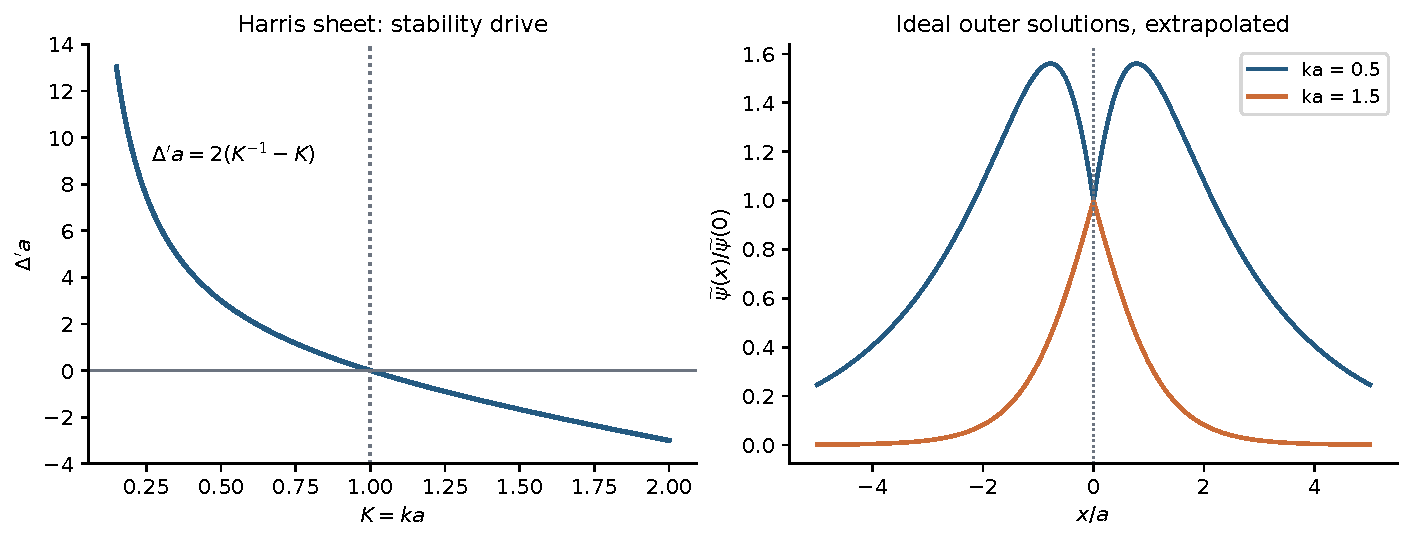
\includegraphics[width=\textwidth]{figures/tm_harris_delta.pdf}
\caption{Harris平衡的解析外区解和$\Delta'a=2(1/K-K)$。中心处折角是忽略内层后得到的两侧渐近解，不是真实无限薄电流奇点；内层将其平滑连接。右图的稳定性判据限定于本章经典无流、无限域问题。}
\label{tm:fig:harris}
\end{figure}

\section{正\texorpdfstring{$\Delta'$}{Delta prime}的物理意义与边界依赖}
当$K<1$时，式\eqref{tm:harrissolution}在中心右侧先向上弯出正斜率，左侧斜率相反。外区希望薄层提供与这种斜率差相容的扰动电流；电阻允许该电流结构随拓扑变化建立，惯性决定流动响应有多快。用“外区提供驱动、内区决定通道和时标”记住分工，比把$\Delta'$只当一个背诵的稳定性符号更有用。

$\Delta'$不是局地点只测$B'_0$就能知道的量。它来自从两侧边界积分到共振面，所以改变导体壁位置、电流剖面、压力曲率或其他共振面，可能改变它甚至改变符号。Harris解析式是一个明确平衡与无限域边界下的结果；不能只因实际磁场在中心近似线性，就对任意装置使用$2(K^{-1}-K)$。

\paragraph{本章学到哪一步。}
现在我们已经知道哪个波长具有经典撕裂驱动，也得到内区必须满足的电流积分。我们\emph{还不知道}$\gamma$与$\delta$。这不是推导缺了一项数值系数，而是外区方程按构造就删掉了决定时标的惯性与电阻；下一章必须把它们取回来。
